\chapter{Introduzione alle reti di calcolatori}

\section{L'importanza delle interconnessioni}
Tutto il mondo è connesso tramite le reti: Internet è la più grande rete di interconnessione esistente,\\ e il suo utilizzo ha stravolto il mondo per com'era conosciuto. 
Le reti velocizzano il trasferimento di dati: ciò avviene tramite un canale fisico, che permette il trasferimento di informazioni secondo dei protocolli stabiliti. Partecipano a queste interconnessioni non solo calcolatori, ma dispositivi (\textit{devices}) di qualsiasi tipo: server, data-center, dispositivi IoT e altro ancora. Data l'importanza delle reti al giorno d'oggi, diventa altrettanto importante \textbf{creare un'infrastruttura solida}, e un \textbf{insieme di protocolli} che assicurino la stabilità del sistema.

\subsection{Cos'è una rete informatica}
È un'infrastruttura che permette di collegare più dispositivi (\textit{devices}), e metterli in comunicazione.\\
Individuiamo due tipi di interconnessioni:
\begin{itemize}
    \item \textbf{Connessione fisica.}\\
    Si riferisce al mezzo fisico (cavo, sistemi wireless).
    \item \textbf{Struttura logica.}\\
    Si riferisce ai protocolli che garantiscono il funzionamento della rete.
\end{itemize}

\newpage

\section{Cos'è un protocollo}\label{1.2.1}
I \textbf{protocolli di rete} sono delle \textbf{regole} che definiscono il \textbf{formato}, e l'\textbf{ordine}, la \textbf{semantica} e la \textbf{sintassi} dei \textbf{messaggi} mandati e ricevuti tra entità interconnesse tramite la rete, nonché le azioni da effettuare per \textbf{garantire un determinato servizio}. Garantire che i \textbf{protocolli} vengano usati dai \textbf{devices} appartenenti a una \textbf{rete} è condizione necessaria per permetterne la \textbf{mutua comunicazione}.

\subsection{Stack di protocolli}
I protocolli di rete differiscono tra loro non solo per le loro caratteristiche, ma anche per il \textbf{livello} di appartenenza negli stack dei protocolli (ISO/OSI, TCP/IP).\\
Ogni protocollo è infatti associato (più o meno rigidamente) ad un livello di uno stack, un'astrazione che ordina insiemi di protocolli dall'alto verso il basso, dipendentemente dal loro ruolo. In \textbf{alto} abbiamo i protocolli più astratti e vicini all'\textbf{utente}, in \textbf{basso} quelli più vicini al \textbf{sistema fisico}. Un messaggio che sfrutta un protocollo del livello più alto, "passa"\footnote{Un esempio? Una richiesta HTTP (protocollo del layer applicativo) sfrutta il protocollo TCP (del layer di trasporto), che sfrutta IP (del layer di rete). Un protocollo del livello $n$-esimo sfrutterà protocolli di tutti i livelli inferiori} attraverso protocolli dei layer inferiori.
Ogni layer aggiunge un \textbf{header} al \textit{payload}, fornendo informazioni specifiche, per permettere la consegna del messaggio e la sua corretta interpretazione.
Il ricevente, infatti, sfrutterà gli header relativi ai vari protocolli (dal basso verso l'alto) per \textbf{interpretare} l'informazione. 

\begin{figure}[htp]
    \centering
    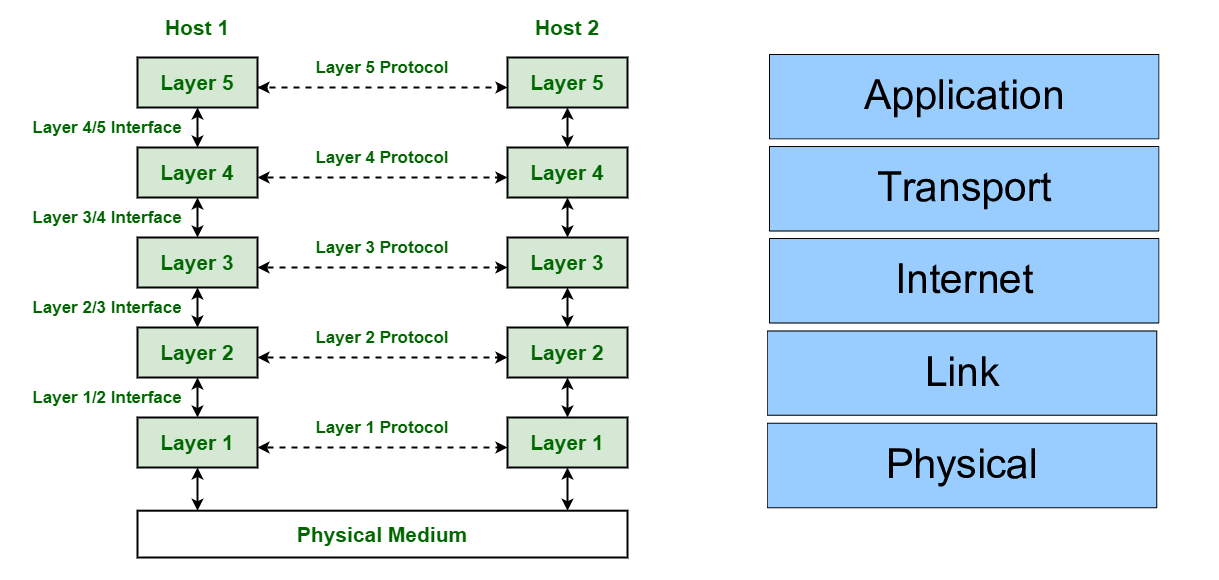
\includegraphics[width=0.9\linewidth]{./images/introduzione.png}
    \caption{Lo stack di nostro riferimento.}
\end{figure}

\subsection{Header}
Un \textbf{header} è un insieme di dati, sotto forma di bitstream, che offrono dati relativi al protocollo di appartenenza. Ogni protocollo, di un dato livello, inserirà un header con dei dati fondamentali per la trasmissione e l'interpretazione del messaggio. 

\subsection{Il mezzo fisico}
È fondamentale che il canale fisico sia gestito in maniera opportuna: il segnale che viene mandato è soggetto alla \textbf{resistenza} del mezzo fisico e alle imperfezioni della rete con conseguenti \textbf{distorsioni}. \\
All'interno del mezzo fisico, ciò che viene trasferito sono informazioni \textbf{logiche} codificate in livelli di tensione \textbf{fisici}: il sistema (solitamente) interpreta un segnale che supera i 2 volt come 1 (True), sotto i 0.8 volt 0 (False). Incluso tra 0.8 e 2 è indeterminato. 

\subsection{Obiettivo}
L'obiettivo, nel costruire l'architettura fisica e la struttura logica di una rete, è quello di ottenere un sistema affidabile (\textit{reliable}) e libero da errori. Nel corso dello studio delle reti, andremo a conoscere molteplici protocolli e meccanismi per aumentare la \textit{reliability} della rete.

\newpage

\section{Tipi di comunicazione}
Un servizio di comunicazione tra host può essere di due tipologie. 
\begin{itemize}
    \item \textbf{Connectionless system.}\\
    Non ha un meccanismo che permette di verificare se l'informazione è arrivata al ricevente (parzialmente o totalmente), e se la connessione è stata stabilita con successo. Il sistema non prevede segnali di ACK (\textit{acknowledgement signal}).
    \item \textbf{Connection oriented.}\\
    Un po' come la doppia spunta blu di WhatsApp, \textbf{un segnale di ACK} ci permette di dare informazioni relative alla ricezione del messaggio da parte del ricevente.
\end{itemize}

\subsection{Connection oriented e le sue criticità}
I sistemi connection oriented offrono informazioni relative alla ricezione del messaggio, ma non sono sempre affidabili. Il segnale di ACK potrebbe essere bloccato (a causa di anomalie e guasti nelle infrastrutture), potrebbe arrivare in ritardo, perdersi o essere mal interpretato.\\
Non è sempre affidabile. La \textit{reliability} è una criticità, la cui gravità aumenta se teniamo presente quanto segue: una rete è usata per collegare dispositivi, e quindi utenti, lontani. Le informazioni sono inviate e ricevute "alla cieca".\\ 
Analogia simpatica: è l'equivalente del "ricevuto" nelle comunicazioni tramite walkie-talkie.

\subsection{Temporizzazione come soluzione}
Se entro un determinato lasso di tempo non si è ricevuto il segnale di ACK relativo alla ricezione di un'informazione, l'informazione viene rimandata.\\
Questo meccanismo permette di \textbf{risolvere le criticità} relative alla comunicazione connection oriented.


\subsection{Topologie di rete}
Esistono due tipi principali di connessione.
\begin{itemize}
    \item \textbf{Point to Point.}\\
    Connessione tramite un canale fisico condiviso esclusivamente tra due dispositivi.
    \item \textbf{Broadcast.}\\
    Connessione tramite un canale fisico condiviso tra più dispositivi. Potrebbe causare collisioni dei pacchetti con conseguenti problemi di distorsione dei dati e impossibile interpretazione dei dati ricevuti.
\end{itemize}

Le reti possono assumere varie topologie:
\begin{itemize}
    \item Reti ad anello.
    \item Reti a stella.
    \item Reti a bus.
\end{itemize}

\subsection{PAN, LAN, MAN, WAN}
Le reti distribuite si differenziano tra loro per l'ampiezza della distribuzione:
\begin{itemize}
    \item \textbf{PAN.}\\
    Personal Area Network, pochi metri di range.
    \item \textbf{LAN.}\\
    Local Area Network, 10 metri, 100 metri o 1 km.
    \item \textbf{MAN.}\\
    Reti che coprono aree metropolitane di raggio dai 10 ai 100km.
    \item \textbf{WAN.}\\
    Ricoprono un'intera nazione, si parla di un raggio che va dai 1000 ai 5000km.
\end{itemize}
Internet è considerabile una WAN (di WAN).
